\documentclass[12pt]{article}

\usepackage[a4paper, margin=25mm]{geometry}

\usepackage{setspace} \onehalfspace

\usepackage[utf8]{inputenc}
\usepackage[T1]{fontenc}

\usepackage{mathptmx}
\usepackage{microtype}
\usepackage{inconsolata}

\usepackage[estonian]{babel}
\addto\captionsestonian{%
  \renewcommand{\refname}{Viidatud kirjandus}%
  \renewcommand{\appendixname}{Lisad}%
}

\usepackage{amsmath} 
\usepackage{amsthm}
\usepackage{amssymb}

\usepackage[labelsep=period]{caption}

\usepackage{array}
\usepackage{tabu}
\usepackage{xspace}

\usepackage{graphicx}
\graphicspath{{figures/}}

\usepackage[hidelinks]{hyperref}
\usepackage[all]{hypcap}

\usepackage{color}
\usepackage{xcolor} 
\definecolor{mauve}{rgb}{0.58,0,0.82}

\usepackage{todonotes}

\usepackage{verbatim}

\usepackage{listings}

\usepackage[style=ieee]{biblatex}
\addbibresource{srcs.bib}

\setlength{\marginparwidth}{2cm}
\newcommand{\TODO}{\todo[inline]}

\usepackage{yquant}
\useyquantlanguage{groups}

\def\nonumsection#1{
    \clearpage\newpage\section*{#1}
    \addcontentsline{toc}{section}{#1}
}

\def\abs#1{\left|#1\right|}

\def\paren#1{\left(#1\right)}

\def\bra#1{\mathinner{\langle#1|}}
\def\ket#1{\mathinner{|#1\rangle}}

\def\cnot{\mathop{\mathrm{CNOT}}}
\def\CNOT{\mathop{\mathrm{CNOT}}}

\def\qft{\mathop{\mathrm{QFT}}\nolimits}

\begin{document}

\tableofcontents

\newpage\nonumsection{Sissejuhatus}

\newpage\section{Kvantarvutus}

Mudeleid kvantavutuseks on mitmeid.
Selles töös kasutame kvantbittidel ja -väravatel põhinevat mudelit, mida kutsutakse ahelamudeliks.

Klassikalist biti tõlgendatakse tõeväärtusena: sellel on kaks võimaliku väärtust \(0\) ja \(1\).
Kvantbitil on võimalike väärtusi lõpmata arv.

Üldiselt on kvantbitt Hilberti ruumi objekti, kuid kitsamalt võib seda käsitleda kompleksse vektorruumi \(\mathbb{C}^2\) objektina.
Iga kvantbiti oleku saab kirja panna superpositsioonina
\begin{align}\label{f:superpos}
    \ket\psi = \alpha\ket0 + \beta\ket1 \rlap{,}
    \qquad\text{kus}\qquad \alpha, \beta \in \mathbb{C}
    \quad\text{ja}\quad \abs{\alpha}^2 + \abs{\beta}^2 = 1
\end{align}
ning \(\ket0\) ja \(\ket1\) on kaks sõltumatud olekut.

Selles töös tähistame
\begin{align}
    \ket0 = \begin{pmatrix}
        0 \\
        1 \\
    \end{pmatrix}
    \qquad\text{ja}\qquad \ket1 = \begin{pmatrix}
        1 \\
        0 \\
    \end{pmatrix} \rlap{,}
\end{align}
mis on antud Pauli \(Z\) operaatori baasis, mida kutsutakse ka (kvant)arvutuslikuks baasiks.

Klassikalised (loogika)väravad teostavad loogikatehteid.
Ühel klassikalisel bitil on võimalik vaid üks unikaalne loogika tehe, kahel bitil juba neli.
Kvant(loogika)väravad teostavad unitaarseid operatsioone, mida kirjeldavad unitaarsed maatriksid.
Kvantväravaid on juba ühe kvantbiti jaoks lõpmata arv.

Ometi leidub mitu sellist kvantväravate komplekti, mille kaudu saab kirja panna kõik teised kvantväravad. 
Ühe sellise univeraalse kompletki moodustavad \(R_x(\theta)\), \(R_y(\theta)\), \(R_z(\theta)\), \(P(\lambda)\) ja \(\CNOT\), mis on toodud tabelis~\ref{tab:gates}, kus need on defineeritud maatrikskujul.
Vähemalt üks univeraalse komplekti värav peab olema kahekvantbitine ja põimiv, antud juhul on selleks \(\CNOT\).

Kõik teised selles töös kasutatavad väravad on samuti toodud tabelis~\ref{tab:gates}, kus need on defineeritud äsjanimetatud universaalse komplekti kaudu, mitte maatrikskujul.

Mõõtmine ei ole unitaarne operatsioon ja seega ei teosta seda kvantvärav.
Tabelis~\ref{tab:gates} pole seda operaatorina tähistatud ega defineeritud.
Samas tähistatakse seda ahelas kvantväravatega sarnaselt.

Mõõtes olekut~\ref{f:superpos} on tõenäosusega \(\abs{\alpha}^2\) tulemuseks \(0\) ja tõenäosusega \(\abs{\beta}^2\) tulemuseks \(1\).
Mitme kvantbiti mõõtmisel on tulemuseks klassikaliste bittide jada.
Üldjuhul tuleb kvantarvuti programmi käitada mitu korda, misjuhul on võimalik leida tulemuste tõenõosusjaotus.

\begin{table}[]
    \centering
    \begin{tabular}{||c|c|c|c||}
        \hline
        Nimetus & Operaatori tähis & Operatori definitsioon & Tähsitus kvantahelas \\
        \hline\hline
        Pööre x-telje sihis & \(R_x(\theta)\) & \(
        \begin{pmatrix}
            \cos\frac{\theta}{2} & -i\sin\frac{\theta}{2} \\
        -i\sin\frac{\theta}{2} & \cos\frac{\theta}{2} \\
        \end{pmatrix}
        \) & \lower6pt\hbox{\begin{tikzpicture}
            \begin{yquant}
                qubit {} q[1];
                box {\(R_x(\theta)\)} q[0];
            \end{yquant}
        \end{tikzpicture}} \\
        Pööre y-telje sihis & \(R_y(\theta)\) & \(
        \begin{pmatrix}
            \cos\frac{\theta}{2} & -\sin\frac{\theta}{2} \\
            \sin\frac{\theta}{2} & \cos\frac{\theta}{2} \\
        \end{pmatrix}
        \) & \lower6pt\hbox{\begin{tikzpicture}
            \begin{yquant}
                qubit {} q[1];
                box {\(R_y(\theta)\)} q[0];
            \end{yquant}
        \end{tikzpicture}} \\
        Pööre z-telje sihis & \(R_z(\theta)\) & \(
        \begin{pmatrix}
            e^{-i\frac{\theta}{2}} & 0 \\
            0 & e^{i\frac{\theta}{2}} \\
        \end{pmatrix}
        \) & \lower6pt\hbox{\begin{tikzpicture}
            \begin{yquant}
                qubit {} q[1];
                box {\(R_z(\theta)\)} q[0];
            \end{yquant}
        \end{tikzpicture}} \\
        Faasioperaator & \(P(\lambda)\) & \(
        \begin{pmatrix}
            1 & 0 \\
            0 & e^{i\lambda} \\
        \end{pmatrix}
        \) & \lower6pt\hbox{\begin{tikzpicture}
            \begin{yquant}
                qubit {} q[1];
                box {\(P(\theta)\)} q[0];
            \end{yquant}
        \end{tikzpicture}} \\
        Juhitud eitus & \(\CNOT\) & \(
        \begin{pmatrix}
            1 & 0 & 0 & 0 \\
            0 & 0 & 0 & 1 \\
            0 & 0 & 1 & 0 \\
            0 & 1 & 0 & 0 \\
        \end{pmatrix}
        \) & \lower6pt\hbox{\begin{tikzpicture}
            \begin{yquant}
                qubit {juhtbitt} ctrl;
                qubit {sihtbitt} trgt;
                cnot trgt | ctrl;
            \end{yquant}
        \end{tikzpicture}} \\
        \hline
        Mõõtmine & --- & --- & \lower6pt\hbox{\begin{tikzpicture}
            \begin{yquant}
                qubit {} q[1];
                measure q[0];
            \end{yquant}
        \end{tikzpicture}} \\
        \hline
    \end{tabular}
    \caption{Operaatorid ja neile vastavad kvantväravad}
    \label{tab:gates}
\end{table}

Kvantahel on operaatorite rakendamise korra kirjeldus.
Joonis~\ref{fig:circuits} on näide kvantahelast.
Igale bitile vastab aheals traat.
Kõik ühel traadil olevad kastid on operaatorid, mis mõjuvad sellele kvantbitile.
Kui kasti läbib mitu traati, mõjub see mitmele kvantbitile.
Juhtbitt on väravaga ühendatud katsutiga, milleks on vertikaalne joon täpiga lõpus.
Väravad on ajalises järjestuses.

\begin{figure}
    \centering
    \begin{tikzpicture}
        \begin{yquant}
            qubit {} q[5];
            box {} q[0];
            box {} (q[1, 2]);
            box {} q[3] | q[2];
            box {} (q[1, 2, 3]) | q[4];
            measure q[0, 1, 2];
        \end{yquant}
    \end{tikzpicture}
    \caption{Kvantahela näide}
    \label{fig:circuits}
\end{figure}

Pikemalt tutvustavad kvantahelamudelit \cite{nielsen+chuang} ja \cite{kaye+laflamme+mosca}.


\newpage\section{Elektronstruktuuri ülesanne}

Selles peatüki teemaks on elektronstruktuuri ülesanne, mis on keskne nii selles töös kui ka kvantkeemias üldiselt.
Esimene etapp selle ülesande lahendamisel on molekulaarse hamiltoniaani ja lainefunktsiooni kuju leidmine, millega selles peatükis tegelemegi.

Esiteks, jaotises~\ref{born-oppeheimer}, lihtsustame üldist molekulaarset hamiltoniaani tehes Born-Oppenheimeri lähenduse.

Järgmisena, jaotises~\ref{hartree+slater}, esitame lainefunktsiooni Slateri determinandina, mis on Hatree korrutise üldistus.

Jaotises~\ref{hatree-fock} lihtsustame hamiltoniaani edasi tehes Hartree-Focki lähenduse.

Viimaks, jaotises~\ref{secquant}, esitame hamiltoniaani teise kvantiseerimise kujul.

Et arvutustamiseks kastuame hiljm valmisteeki, siis esitame siin vaid lahendamise üldskeemi.
Lähtume Szabo ja Ostlundi käsitlusest~\cite{szabo+ostlund}.

\subsection{Molekulaarse süsteemi hamiltoniaan}

Selles töö eesmärgiks on molekuli põhioleku energia leidmine, mis tähendab hamiltoniaani omaväärtuse leidmist.
Selleks on tarvis teada hamiltoniaani kuju.

Hatree ühikutes on molekulaarse süsteemi hamiltoniaani üldkuju
\begin{equation}\label{hgeneric}
    H = \underbrace{-\sum_{i=1}^N\frac{1}{2}\nabla_i^2}_\mathrm{(a)}
        \underbrace{-\sum_{A=1}^M\frac{1}{2M_A}\nabla_A^2}_\mathrm{(b)}
        \underbrace{-\sum_{i=1}^N\sum_{A=1}^M\frac{Z_A}{r_{iA}}}_\mathrm{(c)}
        \underbrace{+\sum_{i=1}^n\sum_{j>i}^N\frac{1}{r_ij}}_\mathrm{(d)}
        \underbrace{+\sum_{A=1}^M\sum_{B>A}^M\frac{Z_AZ_B}{R_{AB}}}_\mathrm{(e)}\rlap{,}
\end{equation}
kus (a) on elektronide kineetilise energia liige, (b) on tuumade kineetilise energia liige, (c) on tuumade ja elektronide tõmbumise liige, (d) on elektronide omavahelise tõukumise liige ja (e) on tuumade omavahelise tõukumise liige.

Valmeis~\eqref{hgeneric} \(r_{ij} = r_i - r_j\), kus \(r_i\) ja \(r_j\) on vastavalt \(i\)-nda ja \(j\)-nda elektroni kohavektorid, ja \(r_{AB} = r_A - r_B\), kus \(r_A\) ja \(r_B\) on vstavalt \(A\)-nda ja \(B\)-nda tuuma kohavektorid.
Teisisõnu, üldkujul sõltub molekulaarse hamiltoniaani nii elektronide kui ka tuumade asukohtadest eksplitsiitselt.

\subsection{Born-Oppenheimeri lähendus}\label{born-oppeheimer}

Born-Oppeheimeri lähendus lubab hamiltoniaani~\eqref{hgeneric} lihtsustada, mis on vajalik arvutusressurside kokku hoidmiseks.

Born-Oppehnimeri lähendus võtab arvesse järgmist.

Tuumad on elektronidega võrreldes peaaegu paigal, sest need on elektronidega võrreldes rasked.
Seega jätame valmeis~\eqref{hgeneric} arvestamata liikme (b).

Elektronid liiguvad tuumade poolt tekitatud väljas, mille võime liikumatute tuumade korral lugeda statsionaarseks.
Sellest johtuvalt jätame valemis~\eqref{hgeneric} arvestamata liikme (e), mis on konstantne ja mille arvestamata jätmisel omafunktsioonid ei muutu.

\TODO{Miks võime (e) arvestamata jätma, kuigi see omaväärtusi mõjutab?}

Lihtsustatud hamiltoniaani
\begin{equation}\label{hborn}
    H = \underbrace{-\sum_{i=1}^N\frac{1}{2}\nabla_i^2}_\mathrm{(a)}
        \underbrace{-\sum_{i=1}^N\sum_{A=1}^M\frac{Z_A}{r_{iA}}}_\mathrm{(c)}
        \underbrace{+\sum_{i=1}^n\sum_{j>i}^N\frac{1}{r_ij}}_\mathrm{(d)}\rlap{,}
\end{equation}
nimetatakse elektrooniliseks hamiltoniaaniks.
Elektroonilise hamiltoniaani jaoks on tuumade kohavektorid parameetrid, eksplitsiitset sõltuvust ei ole.

\TODO{Tekst vajab rohkem tugesid.}

\subsection{Hartree korrutis ja Slateri determinant}\label{hartree+slater}

Hetkel ei võta me arvesse Pauli keeluprintsiipi, kuivõrd me pole üldse arvestanud spinni.
Hamiltoniaan~\eqref{hborn} ei keela mitmel sama spinninga elektronil asuda samas ruumipiirkonnas.

Seega nõutakse, et Schrödingeri võrrandi rahuldamisele lisaks peab fermionide süsteemi lainefunktsioon olema antisümmeetriline.
Peab kehtima
\begin{equation}
    \Psi(x_1,\ldots x_i,\ldots x_j,\ldots x_N)=-\Psi(x_1,\ldots x_j,\ldots x_i,\ldots x_N)
\end{equation}
kus \(x_1\) kuni \(x_N\) on üldised koordinaadid, mis võtavad arvesse nii koordinaate \(r_i\) kui ka spinni \(\omega\).
Antisümmeetria printsiibi kehtimine tagab Pauli keeluprintsiibi kehtimise.

Ühe elektroni auskohta ja spinni kirjeldab spinnorbitaal
\begin{equation}\label{spinorb}
    \chi_i(x_1,\ldots x_N) = \begin{cases}
        \alpha(\omega)\phi_i(r_1,\ldots r_N) & \text{kui \(i\) ei jagu \(2\)-ga,} \\
        \beta(\omega)\phi_i(r_1,\ldots r_N) & \text{kui \(i\) jagub \(2\)-ga,} \\
    \end{cases}
\end{equation}
kus \(i=1,\ldots, K\).
Valemis~\eqref{spinorb} vastab \(\alpha(\omega)\) spinn-üles olukorrale ja \(\beta(\omega)\) spinn-aalla olukorrale.
Funktsioonid \(\phi_i\) on ruumilised orbitaalid, need võtavad arvesse elektroni ruumilist paiknemist.
Ruumiliste orbitaalide arv on üldjuhul lõpmatu, kuid piisav täpsus on võimalik saavutada ka siis, kui võta arvesse vaid \(K\) ruumilist orbitaali, mis peavad katma antud ülesande jaoks olulise alamruumi.

Spinnorbitaalidest saab moodustada Hatree korrutise
\begin{equation}\label{hp}
    \Psi^{HP}(x_1,\ldots x_N) = \chi_i(x_1)\chi_j(x_2)\cdots\chi_k(x_N)\rlap{,}
\end{equation}
\TODO{Szabo ja Ostlundi raamatus on siin vist paremal pool \(x_1\), \(\ldots\) \(x_N\) paksus kirjas, mis on eelnevat arvestades loogiline.}
kus
\begin{equation}
    h(i)\chi_j(x_i) = \epsilon_j \chi_j(x_i)\rlap{.}
\end{equation}
Kui kehtib
\begin{equation}
    H\Psi^{HP}=E\Psi^{HP}\rlap{,}
\end{equation}
siis
\begin{equation}
    E=\epsilon_1+\epsilon_2+\cdots\epsilon_N\rlap{.}
\end{equation}

Siiski on Hatree korrutisel puudused, mistõttu ei saa seda kasutada lainefunktsioonina.
Valemist~\eqref{hp} tulenevalt on
\begin{equation}\label{hp}
    \abs{\Psi^{HP}(x_1,\ldots x_N)}^2dx_1\cdots dx_N = \abs{\chi_i(x_1)}^2dx_1\abs{\chi_j(x_2)}^2dx_2\cdots\abs{\chi_k(x_N)}^2dx_N\rlap{,}
\end{equation}
mis tähendab, et esimese elektroni leidmise tõenäosus \(dx_1\)-ga määratud olekust on sõltumatu teise elektroni leidmise tõenäosusest \(dx_2\)-ga määratud olekust jne.
Samas teame, et ühe elektroni leidmine kindlast ruumipiirkonnast muudab vähem tõenäolisemaks sealtsamast teise sama spinniga elektroni leidmise.
eel enam, Hatree korrutisena kui lainefunktsioon võimaldab öelda, et esimene elektron
on \(dx_1\)-ga määratud orbitaalil, teine elektron on \(dx_2\)-ga määratud orbitaalil jne. Füüsikaliselt lubatav on aga vaid selline lainefunktsioon, mis ei võimalda elektronidel vahet teha.

Hatree korrutise edasiarendus on Slater determinant
\begin{equation}
    \Psi(x_1,\ldots x_N) = \frac{1}{\sqrt{N!}}\begin{pmatrix}
        \chi_i(x_1) & \chi_j(x_1) & \cdots & \chi_k(x_1) \\
        \chi_i(x_2) & \chi_j(x_2) & \cdots & \chi_k(x_2) \\
        \vdots & \vdots & & \vdots \\
        \chi_i(x_N) & \chi_j(x_N) & \cdots & \chi_k(x_N) \\
    \end{pmatrix}\rlap{,}
\end{equation}
millel Hatree korrutise puudusi pole.

\subsection{Hartree-Focki lähendus}\label{hatree-fock}

Ka liikumatute tuumade puhul on \(n > 2\) elektroniga molekulide elektronstruktuuri ülesanne \(n\) keha probleem.
Vajalikuks osutuab Hatree-Focki lähendus, mille järgi üksik elektron liigub tuumade ja teiste elektronide mõju keskmistamisel saadud väljas.

\TODO{Siin peaks olema täpsem sõnastus.}

Varasema põhjal teame, et lainefunktsioon esitub Slateri determinandina.
Variatsiooniprintsiibist tulenevalt on põhioleku lainefunktsioon \(\ket{\Psi_0}\) selline, mille puhul
\begin{equation}
    E_0=\bra{\Psi_0}H\ket{\Psi_0}
\end{equation}
on minimaalne.
Minimeerimine viib Hatree-Focki võrrandini
\begin{equation}
    f(i)\chi(x_i)=\epsilon\chi(x_i)\rlap{,}
\end{equation}
kus
\begin{equation}
    f(i) = -\frac{1}{2}\nabla_i^2-\sum_{A=1}^M\frac{Z_A}{r_{iA}}+\nu^{HF}(i)
\end{equation}
on Focki operaator, milles \(\nu^{HF}(i)\) on on \(i\)-nda elektroni tajutav keskmine teiste elektronide mõjust tulenev potentsiaal.

\TODO{Self-consistent field method.}

Lahendanud Hatree-Focki võrrandi, saadakse \(k\) spinnorbitaali energiateka \(\epsilon_k\).
Nendest spinnorbitaalidest \(N\) madalaima energiaga on täitedetud orbitaalid.
Teised on virutaalssed orbitaalid.

\TODO{Põhioleku lainefunktsiooni kuju.}

\subsection{Teine kvantiseerimine}\label{secquant}

Slateri determindi omadusi, seega antisümmeetria printsiipi, võtab mugavalt arvesse abstraktne teise kvantiseerimise formalism.

Teise kvantsieerimise formalismis esitatakse kõik võimalikud olekud vaakum oleku \(\ket{\mathrm{vak}}\) kaudu.
Defineeritakse tekeoperaator \(a_i^{\dagger}\), mis lisab süsteemi juurde elektroni spinnorbitaalil \(\chi_i\).
Näiteks
\begin{align}
    a_i^{\dagger}\ket{\mathrm{vak}} &= \ket{\chi_i}\rlap{,} \\
    a_j^{\dagger}\ket{\chi_i} & =\ket{\chi_i\chi_j}
\end{align}
jne.
Samuti definereeritakse kaooperaator \(a_i\), mis teeb vastupidist.

Tekke- ja kaooperaatorite omadused on antud nende antikommutatseiooni reeglitega
\begin{equation}
    \left[a_i^{\dagger}, a_j^{\dagger}\right|= 0\rlap{,}
\end{equation}
\begin{equation}
    \left[a_i, a_j\right|= 0\rlap{,}
\end{equation}
ja
\begin{equation}
    \left[a_i^{\dagger}, a_j\right| = \delta_{ij}\rlap{.}
\end{equation}

Tekke- ja kaooperaatorite kaudu saab konstueerida ergastusoperaatori \(X_{i,\ldots, j}^{k,\ldots,l}\), mis tõstab elketronid spinnorbitaalidelt \(i,\ldots,j\) orbitaalidele \(k,\ldots, l\).
Sedasi saab kõik olekud esitada põhioleku kaudu.

\newpage\section{Hamiltoniaan kvantahelana}

Selles peatkükis leiame kvantahela hamiltoniaani simuleerimiseks.
Esmalt teisendame Focki ruumi hamiltoniaani kvantbittide ruumi kasutades Jordan-Wigneri teisendust.
Seejärel kvantbittide ruumi hamiltoniaani kvantahelana.

\subsection{Jordan-Wigneri teisendus}

\TODO{Neutraalsem sõnastus!}

Soovime kvantahelana realiseerida operaatorit
\begin{equation}\label{eq:hamtime}
  U = e^{-iHt}\rlap{,}
\end{equation}
kus \(H\) on hamiltoniaan.
Varasemalt käsitlesime hamiltoniaani \(H\) Focki ruumi operaatorina.
Jordan-Wigneri teisendus~\cite{jordan+wigner} lubab meil \(H\) üle viia kvantbittide ruumi~--- see on esimene samm operaatori \(U\) esitamiseni kvantahelana.

Siin töös me Jordan-Wigneri teisenduse üksikasju ei käsitle, kuid toome ära mõned selle kasulikud omadused.

Esiteks, selle teisenduse tulemusena saame hamiltoniaani \(H\) Pauli sõnede summana~\cite{whitfield+etal}.
Pauli sõnede all mõistame Pauli maatriksite tensorkorrutisi.
Sümboolselt
\begin{equation}\label{eq:paulisum} H = \sum_i h_i\rlap{,} \end{equation}
kus $h_i$ on Pauli sõne.

Edaspidi tähistame Pauli sõnesesid lühidalt
\begin{equation} h_i=P_{j_1}P_{j_2}\cdots P_{j_k} \rlap{,}\end{equation}
kus \(j_1\), \(j_2\), $\ldots$, \(j_k\) tähistavad kvantbitte, millele \(P_{j_1}\), \(P_{j_2}\), \(\ldots\), \(P_{j_k}\in\{X,Y,Z\}\) mõjuvad.
Näiteks \(X_1Y_2Z_4=X\otimes Y\otimes 1\otimes Z.\)
(Selles tähistuses peab Pauli sõne dimensioon olema selge kontekstist, sest viimase Pauli X-, Y- või Z-maatrikisi järel võib olla kuitahes palju ühikmaatrikseid.)

Teiseks, võimalikele puhastele olekutele vastavad vektorid kujul
\begin{equation}
  \ket{x_1x_2\cdots x_n}
     = \ket{x_1}\otimes\ket{x_2}\otimes\cdots\otimes\ket{x_n}\rlap{,}
\end{equation}
kus $x_1$, $x_2$, $\ldots$ $x_n\in\{0,1\}$ näitab spinnorbitaalide $1$, $2$, $\ldots$, $n$ täidetust ja $n$ on spinnorbitaalide arv süsteemis~[viide?].
Näiteks, kvantbittide ruumi seisund \(\ket{\Psi_0}=\ket{1100}\) vastab Focki ruumi seisundile, kus alumised kaks spinnorbitaali on täidetud ja ülemised kaks mitte~\cite{szabo+ostlund, mcardle+etal}.

\subsection{Pauli \(Z\) maatriksite tensorkorrutise eksponent}

Soovime kvantahelana realiseerida operaatorit~\ref{eq:hamtime}.
Vaatame kõigepealt lihtsat juhtu.
Kui
\begin{equation}
  H=Z_{j_1}Z_{j_2}\cdots Z_{j_n}\rlap{,}
\end{equation}
siis operaatorit~\ref{eq:hamtime} realiseerib kvantahel joonisel~\ref{f:expz}.

\begin{figure}[h]
  \centering
  \begin{tikzpicture}
    \begin{yquant}
      qubit {$j_1\colon$} q[1];
      qubit {$j_2\colon$} q[+1];
      qubit {} q[+1]; discard q[2];
      qubit {$j_{n-1}\colon$} q[+1];
      qubit {$j_n\colon$} q[+1];
      cnot q[4] | q[0];
      cnot q[4] | q[1];
      text {$\ \ldots\ $} q[0,1,3,4];
      cnot q[4] | q[3];
      box {$R_z(2t)$} q[4];
      cnot q[4] | q[3];
      text {$\ \ldots\ $} q[0,1,3,4];
      cnot q[4] | q[1];
      cnot q[4] | q[0];
    \end{yquant}
  \end{tikzpicture}
  \caption{Operaatori \(e^{-iZ_{j_1}Z_{j_2}\cdots Z_{j_n}t}\) realiseerimine kvantahelana. Bitte, mis \(j_1\), \(j_2\), \(\cdots\), \(j_n\) hulgas ei esine, pole näidatud}
  \label{f:expz}
\end{figure}

Teisisõnu, bitile \(j_n\) tuleb järjest rakenda bittide \(j_1\), \(j_2\), \(\cdots\), \(j_{n-1}\) juhitud \(\cnot\)-väravavaid.
Siis tuleb bitti \(j_n\) pöörata väravaga \(R_z(2a)\).
Viimaks tuleb bitile \(j_n\) järjest rakendada bittide \(j_{n-1}\), \(j_{n-2}\), \(\cdots\), \(j_1\) jihtud \(\cnot\)-väravaid.
Bitte, mis \(j_1\), \(j_2\), \(\cdots\), \(j_n\) hulgas ei esine, ei mõjutata~\cite{mansky+etal}.

Kesksele väravale \(R_z(2a)\) eelnev \(\cnot\)-väravate osa arvutab bitide \(j_1\), \(j_2\), \(\cdots\), \(j_n\) paarsuse.
Keskne värav \(R_z(2a)\) teeb sobiva pöörde.
Järgnev \(\cnot\)-väravate osa kustutab ära nüüdseks ebavajaliku informatsiooni paarsuse kohta~\cite{nielsen+chuang}.

\subsection{Pauli \(X\), \(Y\) ja \(Z\) maatriksite tensorkorrutise eksponent}

Vaatame nüüd keerukamat juhtu, kus \(H\) on Pauli X-, Y- ja Z-maatriksite tensorkorrutis, mitte vaid Z-maatriksite tensorkorrutis.
Näiteks, olgu
\begin{equation}
  H=Z_1X_2Y_3\rlap{.}
\end{equation}

Ahela koostamiseks kasutame ära asjaolu, et
\begin{equation} Z=HXH \end{equation}
ja
\begin{equation} Z=S^{\dagger}HYHS\rlap{.} \end{equation}
Järeldame, et \(e^{-iZ_1X_2Y_3}\) ahel on võimalik saada \(e^{-iZ_1Z_2Z_3}\) ahelast sobivate baasiteisendustega.
Sobiv ahel on joonisel~\ref{f:zxyex}~\cite{nielsen+chuang}.

\begin{figure}[h]
  \centering
  \begin{tikzpicture}
    \begin{yquant}
      qubit {$1\colon$} q[1];
      qubit {$2\colon$} q[+1];
      qubit {$3\colon$} q[+1];
      box {$H$} q[1];
      box {$S^{\dagger}$} q[2];
      box {$H$} q[2];
      cnot q[2] | q[0];
      cnot q[2] | q[1];
      box {$R_z(2t)$} q[2];
      cnot q[2] | q[1];
      cnot q[2] | q[0];
      box {$H$} q[1];
      box {$H$} q[2];
      box {$S$} q[2];
    \end{yquant}
  \end{tikzpicture}
  \caption{\(e^{-iZ_1X_2Y_3}\) realiseerimine kvantahelana}
  \label{f:zxyex}
\end{figure}

\subsection{Pauli sõnede summade eksponent}

Üldjuhul on hamiltoniaan Pauli sõnede summa~\ref{eq:paulisum}.
Kui summa liikmed kommuteeruvad, siis võime kirjutada
\begin{equation}
  e^{-i\sum_i h_it}=\prod_ie^{-ih_it}\rlap{,}
\end{equation}
enamasti see aga nii ei ole.

On näidatud, et
\begin{equation}
  e^{-i\sum_i h_it}=\lim_{\Delta t\rightarrow0}\paren{\prod e^{-ih_i t/\Delta t}}^{\Delta t}
\end{equation}
ka mittekommuteeruvate summa liikmete $h_i$ puhul.
Seega lõpliku $\Delta t$ puhul
\begin{equation}
  e^{-i\sum_i h_it}\approx\paren{\prod e^{-ih_i t/\Delta t}}^{\Delta t}\rlap{,}
\end{equation}
kus paras $\Delta t$ väärtus tuleb enamasti leida eksperimentaalselt.
Seda meetodit ahela koostamiseks nimetatakse Suzuki-Trotteri lahutuseks või lihtsalt trotteriseerimiseks~\cite{mansky+etal}

\TODO{Kas käsitleda ka kontrollitud operaatorite realiseerimist kvantahelana?}

\newpage\section{Faasi hindamine}

Selles peatükis tutvume faasi hindamise algoritmiga, mille abil on võimalik leida unitaarse operaatori faasi.
Esmalt vaatame kvantarvutuslikui Fourier' teisendust ja pöördteisendust, mis on faasi hindamise algoritmi üks osa.
Siis vaatame faasi hindamise algoritmi ennast.
Lõpuks vaatame, kuidas on faasi hindamise algoritmi abil võimalik leida ka hermiitilise operaatori omaväärtusi.

\subsection{Kvantarvutuslik Fourier' teisendus ja pöördteisendus}

Kvantarvutusliku Fourier' teisenduse definitsiooni kohaselt
\begin{equation}
    \qft\colon
    \ket j \mapsto \frac{1}{\sqrt{2^n}}\sum_{k=0}^{2^n-1}e^{2\pi ijk/2^n}\ket k\rlap{,}
\end{equation}
kus \(\ket j\) ja \(\ket k\) on \(n\)-bitised baasivektorid.
See teisendus on linaarne, mis tähendab, et võime oma käsitluses keskenduda vaid mõjule baasivektoritele.

\begin{figure}[h]
    \centering
    \begin{tikzpicture}[scale=0.8]
        \begin{yquant}
            qubit {\(\ket{j_1}\)} q[1];
            qubit {\(\ket{j_2}\)} q[+1];
            qubit {\(\vdots\)} q[+1]; discard q[2];
            qubit {\(\ket{j_{n-1}}\)} q[+1];
            qubit {\(\ket{j_n}\)} q[+1];

            h q[0];
            box {\(P(2\pi/2^2)\)} q[0] | q[1];
            text {\(\ \ldots\ \)} q[0, 1, 3, 4];

            h q[1];
            text {\(\ \ldots\ \)} q[0, 1, 3, 4];
            box {\(P(2\pi/2^{n-2})\)} q[1] | q[3];
            box {\(P(2\pi/2^{n-1})\)} q[1] | q[4];

            text {\(\ \ldots\ \)} q[0, 1, 3, 4];
            h q[3];
            box {\(P(2\pi/2^2\)} q[3] | q[4];

            h q[4];

            swap (q[0, 4]);
            swap (q[1, 3]);

            output {\(\frac{\ket0+e^{2\pi0.j_n}\ket1}{\sqrt{2}}\)} q[0];
            output {\(\frac{\ket0+e^{2\pi0.j_{n-1}j_n}\ket1}{\sqrt{2}}\)} q[1];
            output {\(\vdots\)} q[2];
            output {\(\frac{\ket0+e^{2\pi0.j_2\cdots j_n}\ket1}{\sqrt{2}}\)} q[3];
            output {\(\frac{\ket0+e^{2\pi0.j_1\cdots j_n}\ket1}{\sqrt{2}}\)} q[4];
        \end{yquant}
    \end{tikzpicture}
    \caption{Kvantarvutusliku Fourier' teisneduse ahel}
    \label{fig:qft}
\end{figure}

Näitame, et kvantarvutusliku Fourier' teisenduse sab realiseerida ahelaga~\ref{fig:qft}.

Kasutame siin tähistust, kus
\begin{equation}
    0.j_1j_2\cdots j_n=j_12^{-1}+j_22^{-2}+\cdots+j_n2^{-n}\rlap{.}
\end{equation}

Defineerima Hadamardi operaatori
\begin{equation}
    H = R_x(\pi)R_y(\pi/2) = \frac{1}{\sqrt{2}}\begin{pmatrix}
        1 & 1 \\
        1 & -1 \\
    \end{pmatrix}\rlap{.}
\end{equation}
\TODO{Võrdusmärk pole siin päris õige, sest arvestada tuleb ka globaalset faasi.}
Selle mõju baasivektoritele on
\begin{equation}\label{f:hzero}
    H\ket0=\frac{\ket0 + \ket1}{\sqrt{2}}\rlap{,}
\end{equation}
\begin{equation}\label{f:hone}
    H\ket1=\frac{\ket0 - \ket1}{\sqrt{2}}\rlap{.}
\end{equation}
Valemid \eqref{f:hzero} ja \eqref{f:hone} saab kokkuvõtta valemiks
\begin{equation}\label{f:huseful}
    H\ket{j_i} = \frac{\ket0 + 2^{2\pi j_i}\ket1}{\sqrt{2}}\rlap{.}
\end{equation}

Samuti defineerimie faasi operaatori
\begin{equation}
    P(\lambda) = R_z(\lambda)\rlap{.}
\end{equation}
Mõju baasivektoritele on
\begin{equation}\label{f:pzero}
    P(\lambda)\ket0=\ket0\rlap{,}
\end{equation}
\begin{equation}\label{f:pone}
    P(\lambda)\ket1=e^{i\lambda}\ket1\rlap{.}
\end{equation}
Valemitest \eqref{f:pzero} ja \eqref{f:pone} järeldub kasulik omadus
\begin{equation}\label{f:puseful}
    P(2\pi 0.0j_2)\frac{\ket0+e^{2\pi i0.j_1}\ket1}{\sqrt{2}}) =\frac{\ket0+e^{2\pi i0.j_1j_2}\ket1}{\sqrt{2}})
\end{equation}

Olgu algolek
\begin{equation}
    \ket j = \ket{j_1}\otimes\ket{j_2}\otimes\cdots\otimes\ket{j_n}
\end{equation}
kus \(j_1\), \(j_2\), \(\ldots\), \(j_n \in \{0, 1\}\) on \(j\) kohad kahendsüsteemis (\(j_1\) on kõrgeim koht).

Järgime skeemi~\ref{fig:qft}.

\TODO{Korduv lauseskeem:}

Mõjunud esimesele bitile Hadamardi operaatoriga \(H\), on süsteem olek
\begin{equation}
    \frac{\ket0+e^{2\pi i0.j_1}\ket1}{\sqrt{2}}\otimes\ket{j_2}\otimes\cdots\otimes\ket{j_n}\rlap{,}
\end{equation}
tulenevalt valemist~\eqref{f:huseful}.


Mõjunud esimesele bitile faasiväravaga \(P(2\pi 0.0j_2\) juhinduvalt teisest bitist, on süsteemi olek
\begin{equation}
    \frac{\ket0+e^{2\pi i0.j_1j_2}\ket1}{\sqrt{2}}\otimes\ket{j_2}\otimes\cdots\otimes\ket{j_n}\rlap{,}
\end{equation}
tulenevalt valemist~\eqref{f:puseful}.

Mõjunud esimesele bitile faasiväravaga \(P(2\pi 0.00j_3\) juhinduvalt kolmandast bitist, on süsteemi olek
\begin{equation}
    \frac{\ket0+e^{2\pi i0.j_1j_2j_3}\ket1}{\sqrt{2}}\otimes\ket{j_2}\otimes\cdots\otimes\ket{j_n}\rlap{.}
\end{equation}
sarnaselt eelmise sammuga.

Sedasi jätkanud, on süsteem olek
\begin{equation}
    \frac{\ket0+e^{2\pi i0.j_1j_2\cdots j_n}\ket1}{\sqrt{2}}\otimes\ket{j_2}\otimes\cdots\otimes\ket{j_n}\rlap{.}
\end{equation}

Toiminud teise bitiga samuti nagu esimesega, on süsteemi olek
\begin{equation}
    \frac{\ket0+e^{2\pi i0.j_1j_2\cdots j_n}\ket1}{\sqrt{2}}\otimes
    \frac{\ket0+e^{2\pi i0.j_2j_3\cdots j_n}\ket1}{\sqrt{2}}
    \otimes\ket{j_3}\otimes\cdots\otimes\ket{j_n}\rlap{.}
\end{equation}

Toiminud ülejäänud bittidega niisamuti, on süsteemi olek
\begin{equation}
    \frac{\ket0+e^{2\pi i0.j_1j_2\cdots j_n}\ket1}{\sqrt{2}}\otimes
    \frac{\ket0+e^{2\pi i0.j_2j_3\cdots j_n}\ket1}{\sqrt{2}}
    \otimes\cdots\otimes
    \frac{\ket0+e^{2\pi i0.j_n}\ket1}{\sqrt{2}}\rlap{.}
\end{equation}
Avanud sulud ja koondanud,
\begin{equation}
    \frac{1}{\sqrt{2^n}}\sum_{k=0}{2^n-1}e^{2\pi ijk/2^n}\ket k\rlap{,}
\end{equation}
mis ongi Fourier' teisenduse tulemus.

Kvantarvutusliku Fourier' pöördteisenduse definitsiooni kohaselt
\begin{equation}
    \qft^{-1}\colon
    \frac{1}{\sqrt{2^n}}\sum_{k=0}^{2^n-1}e^{2\pi ijk/2^n}\ket k \mapsto \ket j\rlap{,}
\end{equation}
Pöördteisenduse ahela saame teisenduse ahela pööramisel.
Selleks tuleb läbida eelnev arutelu tagant ette asendades operaatorid pöördoperaatoritega.
Hadamardi operaator \(H\) on iseenda pöördoperaator.
Faasioperaatori \(P(\lambda)\) pöördoperaator on \(P(-\lambda)\)

\TODO{Ehk oleks loogilisem tutvustada pikemalt \(\qft^{-1}\)-d, mitte \(\qft\)-d.}

\subsection{Unitaarse operaatori omaväärtusülesanne}

Kehtib
\begin{equation}\label{eq:unitarypea}
    U\ket u=e^{2\pi i\phi}\ket u\rlap{,}
\end{equation}
kus \(U\) on unitaarne operaator, \(\ket u\) selle omavektor ja \(e^{2\pi i\phi}\) vastav omaväärtus ehk faas ning \(\phi=0.\phi_1\phi_2\cdots\phi_n\).
Kujust tulenevalt \(0\le\phi<1\).
Soovime hinnata \(U\) faasi, milleks piisab, kui leiame \(\phi\) väärtuse.
See on faasi hindamise ülesanne.

Näitame, et selle ülesande lahendamiseks sobib ahel~\ref{fig:pea}.

\begin{figure}[h]
    \centering
    \begin{tikzpicture}
        \begin{yquant}
            qubit {$\ket0$} pea[1];
            qubit {$\ket0$} pea[+1];
            qubit {$\vdots$} pea[+1]; discard pea[2];
            qubit {$\ket0$} pea[+1];
            qubit {$\ket0$} pea[+1];

            qubit {$\ket u$} state;

            box {$\mathop{\rm QFT}$} (pea[0], pea[1], pea[2], pea[3], pea[4]);

            box {$U^{2^0}$} state | pea[4];
            box {$U^{2^1}$} state | pea[3];
            text {$\ \ldots\ $} pea[0], pea[1], pea[3], pea[4], state;
            box {$U^{2^{n-2}}$} state | pea[1];
            box {$U^{2^{n-1}}$} state | pea[0];

            box {$\mathop{\rm QFT}\nolimits^{-1}$} (pea[0], pea[1], pea[2], pea[3], pea[4]);
            measure pea[0], pea[1], pea[3], pea[4];
            output {$\phi_1$} pea[0];
            output {$\phi_2$} pea[1];
            output {$\vdots$} pea[2];
            output {$\phi_{n-1}$} pea[3];
            output {$\phi_n$} pea[4];
            output {$\ket u$} state;
        \end{yquant}
        \end{tikzpicture}
    \caption{Kvantahel \(U\) faasi hindamiseks}
    \label{fig:pea}
\end{figure}

Meil on kaks registrit

Üks neist on faasi hindamise register, kus on \(n\) bitti.
Eeldame, et faasi hindamise registris on nii palju bitte, kui on vaja \(\phi\) esitamiseks.

Teine on olekuregister, mille bittide arv pole oluline.
Joonisel~\ref{fig:pea} on olekuregistrit tähistatud ühe traadiga, kuid bitte võib selles registris olla rohkem kui üks.

Algselt on faasi hindamise registri kõik kvantbiti olekus \(\ket 0\).
Mõjunud neile Fourier' teisenduse operaatoriga, on kõik faasi hindamise registri kvantbitid olekus
\begin{equation}
    \frac{\ket0+\ket1}{\sqrt{2}}\rlap{.}
\end{equation}

Mõjunud olekuregistrile operaatoriga \(U^{2^0}\) juhinduvalt faasi hindamise registri kvantbitist \(n\), on süsteemi kui terviku olek
\begin{equation}
    \frac{\ket0+\ket1}{\sqrt{2}}\otimes
    \cdots\otimes
    \frac{\ket0+\ket1}{\sqrt{2}}\otimes
    \frac{\ket0+e^{2\pi i2^0\phi}\ket1}{\sqrt{2}}\otimes
    \ket u\rlap{.}
\end{equation}

\TODO{Siin peaks mainima faasi tagasi löömise efekti.}
\TODO{Parem lausestruktuur.}

Mõjunud olekuregistrile operaatoriga \(U^{2^1}\) juhinduvalt teiseste faasi hindamise registri kvantbitist, on süsteemi olek
\begin{equation}
    \frac{\ket0+\ket1}{\sqrt{2}}\otimes
    \cdots\otimes
    \frac{\ket0+\ket1}{\sqrt{2}}\otimes
    \frac{\ket0+e^{2\pi i2^1\phi}\ket1}{\sqrt{2}}\otimes
    \frac{\ket0+e^{2\pi i2^0\phi}\ket1}{\sqrt{2}}\otimes
    \ket u\rlap{.}
\end{equation}

Nõnda jätkatanud,
\begin{equation}
    \frac{\ket0+e^{2\pi i2^{n-1}\phi}\ket1}{\sqrt{2}}\otimes
    \frac{\ket0+e^{2\pi i2^{n-2}\phi}\ket1}{\sqrt{2}}\otimes
    \cdots\otimes
    \frac{\ket0+e^{2\pi i2^0\phi}\ket1}{\sqrt{2}}\otimes
    \ket u\rlap{.}
\end{equation}
Varasema põhjal on viimane seisnud sama, mis
\begin{equation}
    \frac{\ket0+e^{2\pi i0.\phi_n}\ket1}{\sqrt{2}}\otimes
    \frac{\ket0+e^{2\pi i0.\phi_{n-1}\phi_n\phi}\ket1}{\sqrt{2}}\otimes
    \cdots\otimes
    \frac{\ket0+e^{2\pi i2^0.\phi_1\phi_2\cdots\phi_n}\ket1}{\sqrt{2}}\otimes
    \ket u\rlap{.}
\end{equation}

Rakendanud faasi hindamise registrile Fourier' pöörteisenduse operaatorit, on süsteemi olek
\begin{equation}
    \ket{\phi_0}\otimes\ket{\phi_2}\otimes\cdots\otimes\ket{\phi_n}\ket{u}\rlap{.}
\end{equation}
Mõõtnud faasi hindamise registri kvantbitte, saame klassikaliste bittide jada
\begin{equation}
    \phi_1, \phi_2, \ldots, \phi_n\rlap{,}
\end{equation}
mille põhjal saab leida \(\phi=0.\phi_1\phi_2\cdots\phi_n\).

Arutlesime eeldusel, et faasi hindamise registris on sama palju bitte \(n\), kui on vaja \(\phi=0.\phi_1\phi_2\cdots\phi_,\) esindamiseks kahendüssteemis \(m = n\).

Kui võtta \(n > m\), siis jääb eelnev arutelu kehtima, ainult et \(\phi_{m+1}\), \(\phi_{m+2}\), \(\ldots\), \(\phi_n = 0\).

On näidatud, et juhul \(n < m\) on \(0.\phi_1\phi_2\cdots\phi_n\) suurima täenäosusega \(\phi\) hinnang \(n\)-bitise täpsusega.
Maksimaalne viga on \((1/2)/2^{n+1}\).

\TODO{Viimane arutelu tuleks kindlasti paremini sõnastada.}

\subsection{Hermiitilise operaatori omaväärtusülesanne}

Selles töös soovime leida hamiltonaani omaväärtusi.
Nüüdseks oskame leida unitaarse operaatori omaväärtusi, kuid hamiltoniaan pole üldjuhul unitaarne operaator.
See-eest on hamiltoniaan hermeetiline.
Näitame, et hermeetilise operaatori omaväärtuste leidmine taandub unitaarse operaatori omaväärtuste leidmisele.
Teeme seda hamiltoniaani näitel.

Et hamiltoniaan \(H\) on hermeetiline, siis ajalise arengu operaator
\begin{equation}
    U=e^{-iHt}\rlap{,}
\end{equation}
on unitaarne, kusjuures \(t\) on reaalne kordaja, mille vajalikkus selgub hiljem.

Kehtib
\begin{equation}
    U\ket{E_n}=e^{-iHt}\ket{E_n}=e^{-iE_nt}\ket{E_n}
\end{equation}
\TODO{Kas seda oleks vaja näidata?}
Võime võtta \(E_n t=2\pi\phi\), millega oleme jõudnud valemini~\ref{eq:unitarypea}.

Et \(0 \le \phi < 1\), siis peame \(t\) valima nii, et
\begin{equation}
    0 \le E_nt < 2\pi\rlap{.}
\end{equation}
Seega
\begin{equation}
    T = \frac{2\pi}{E_\mathrm{piir}}\rlap{,}
\end{equation}
kus \(E_\mathrm{piir} \ge E_n\).

\TODO{Viimane arutelu peaks olema vähev uitav.}

\newpage\section{Metoodika}

Selles peatükis võtame kokku protseduuri molekuli põhienergia leidmiseks.
Samuti tutvustame vahendeid arvutuste läbiviimiseks.

\subsection{Lahendamise skeem}

Esitame nüüd molekulaarse hamiltonaani energia leidmise sammud.

Ülesande lahendamine algab molekuli geomeetria kirja panemisest.
Tuleb määrata aatomite koosseis molekulis ja aatomite vahelised kaugused.
Samuti tuleb valida keemiline baas.
Sealt edasi saab leida konkreetse molekuli hamiltoniaani kuju.
Hamiltoniaani tuleb seejärel lihtsustada Born-Oppenheimeri ja Hatree-Focki lähenduses.
Lõpuks tuleb hamiltonaain esitada teise kvantiseerimise kujul.

Samuti tuleb leida huvipakkuvale olekule võimalikult lähedane olek Hartree korrutisena.

Järgmisena tuleb Focki ruumi hamiltoniaan esitada kvantbittide ruumis.
Selleks saab kasutada Jordan-Wigneri teisendust.
Järgmiseks tuleb kvantahelana realiseerida operaator, mis on hamiltoniaani eksponent.
Et hamiltoniaan on pärast Jordan-Wigneri teisendust Pauli sõnede summa, siis leidub skeem selle esitamiseks kvantahalana, kuid seda võib olla vaja trotteriseerida.

Faasihindamise jaoks on oluline, et unitaarne operaator oleks juhitud.
Juhitud unitaarse operaatori saab kui kvantahelas asendada kõik pöörded juhitud pööretega.
Nõnda toiminud, sõltub iga Pauli sõne rakendamine sellest, mis on juhtkvantbiti olek.
Kui juhtkvantbitt on olekus \(\ket0\), pööre ei rakendu.
Et paarsuse arvutamine ja selle tagasi panemine on pöördoperatsioonid, siis kokkuvõttes antud Pauli sõne justkui ei rakendu.
Kui juhtkvantvitt on olekus \(\ket1\) pööre rakendub ja rakendub ka Pauli sõne tervikuna.

Eraldi tuleb arvestada hamiltoniaani seda liiget, mis on ühikmaatriksite tensorkorrutis.
Sellise liikme eksponent on globaalse faasi operaator, mille juhtimiseta juhul võib jätta arvestamata.
Samas juhitud globaalse faasi operaator rakendaine muudab suhtelise faasi ja seda peab arvestama.
Juhtitud globaalse faasi operaatori võib asendanda juhtkvantvitil rakendatud suhtelise faasi opetaatoriga, nagu näha joonisel~\ref{fig:globphase}.

\begin{figure}[h]
    \centering
    \begin{tikzpicture}
        \begin{yquantgroup}
            \registers{
                qubit {} q[2];
            }
            \circuit{
                box {\(GP(\alpha)\)} q[1] | q[0];
            }
            \equals
            \circuit{
                box {\(P(-\alpha)\)} q[0];
            }
        \end{yquantgroup}
    \end{tikzpicture}
    \caption{Juhitud globaalse faasi operaaotri saab asendada juhtkvantbitile rakendatud faasi operaatoriga, mille argument peab olema vastupidine~\cite{nielsen+chuang}}
    \label{fig:globphase}
    \TODO{Üks traat on puudu}
\end{figure}

Viimaks tuleb koostada faasi hindamise kvantahel ja seda käitada.
Trotteriseerimise sammude arv ja faasi hindamise registri suurus tuleb valida sobivalt.

\TODO{Kas siin peaks olema lahendamise skeem joonisena?}

\subsection{Kasutatud vahendid}

Töös kasutsime programmeerimiskeelt Python.

Geomeetriast hamiltonaani saamist ja Jordan-Wigneri teisendust võimaldas teek OpenFermion~\cite{openfermion}.

Kvantahela koostamiseks ja selle klassikaliseks simuleerimiseks kasutasime teeki Qiskit~\cite{qiskit}.

Trotterisammude arvu, faasi hindamise registri suuruse ja energia piirväärtuse valikut selgitab järgmine peatükk.
Keemiliseks baasiks võtsime STO-3G.

\newpage\section{Tulemused}

\subsection{Vesiniku molekuli energia}

Selles töös võtsime mudelsüsteemiks \(\mathrm{H}_2\) molekuli.
STO-3G baasis on selle molekuli hamiltoniaan neljakvantbitine.

\begin{figure}[h]
    \centering
    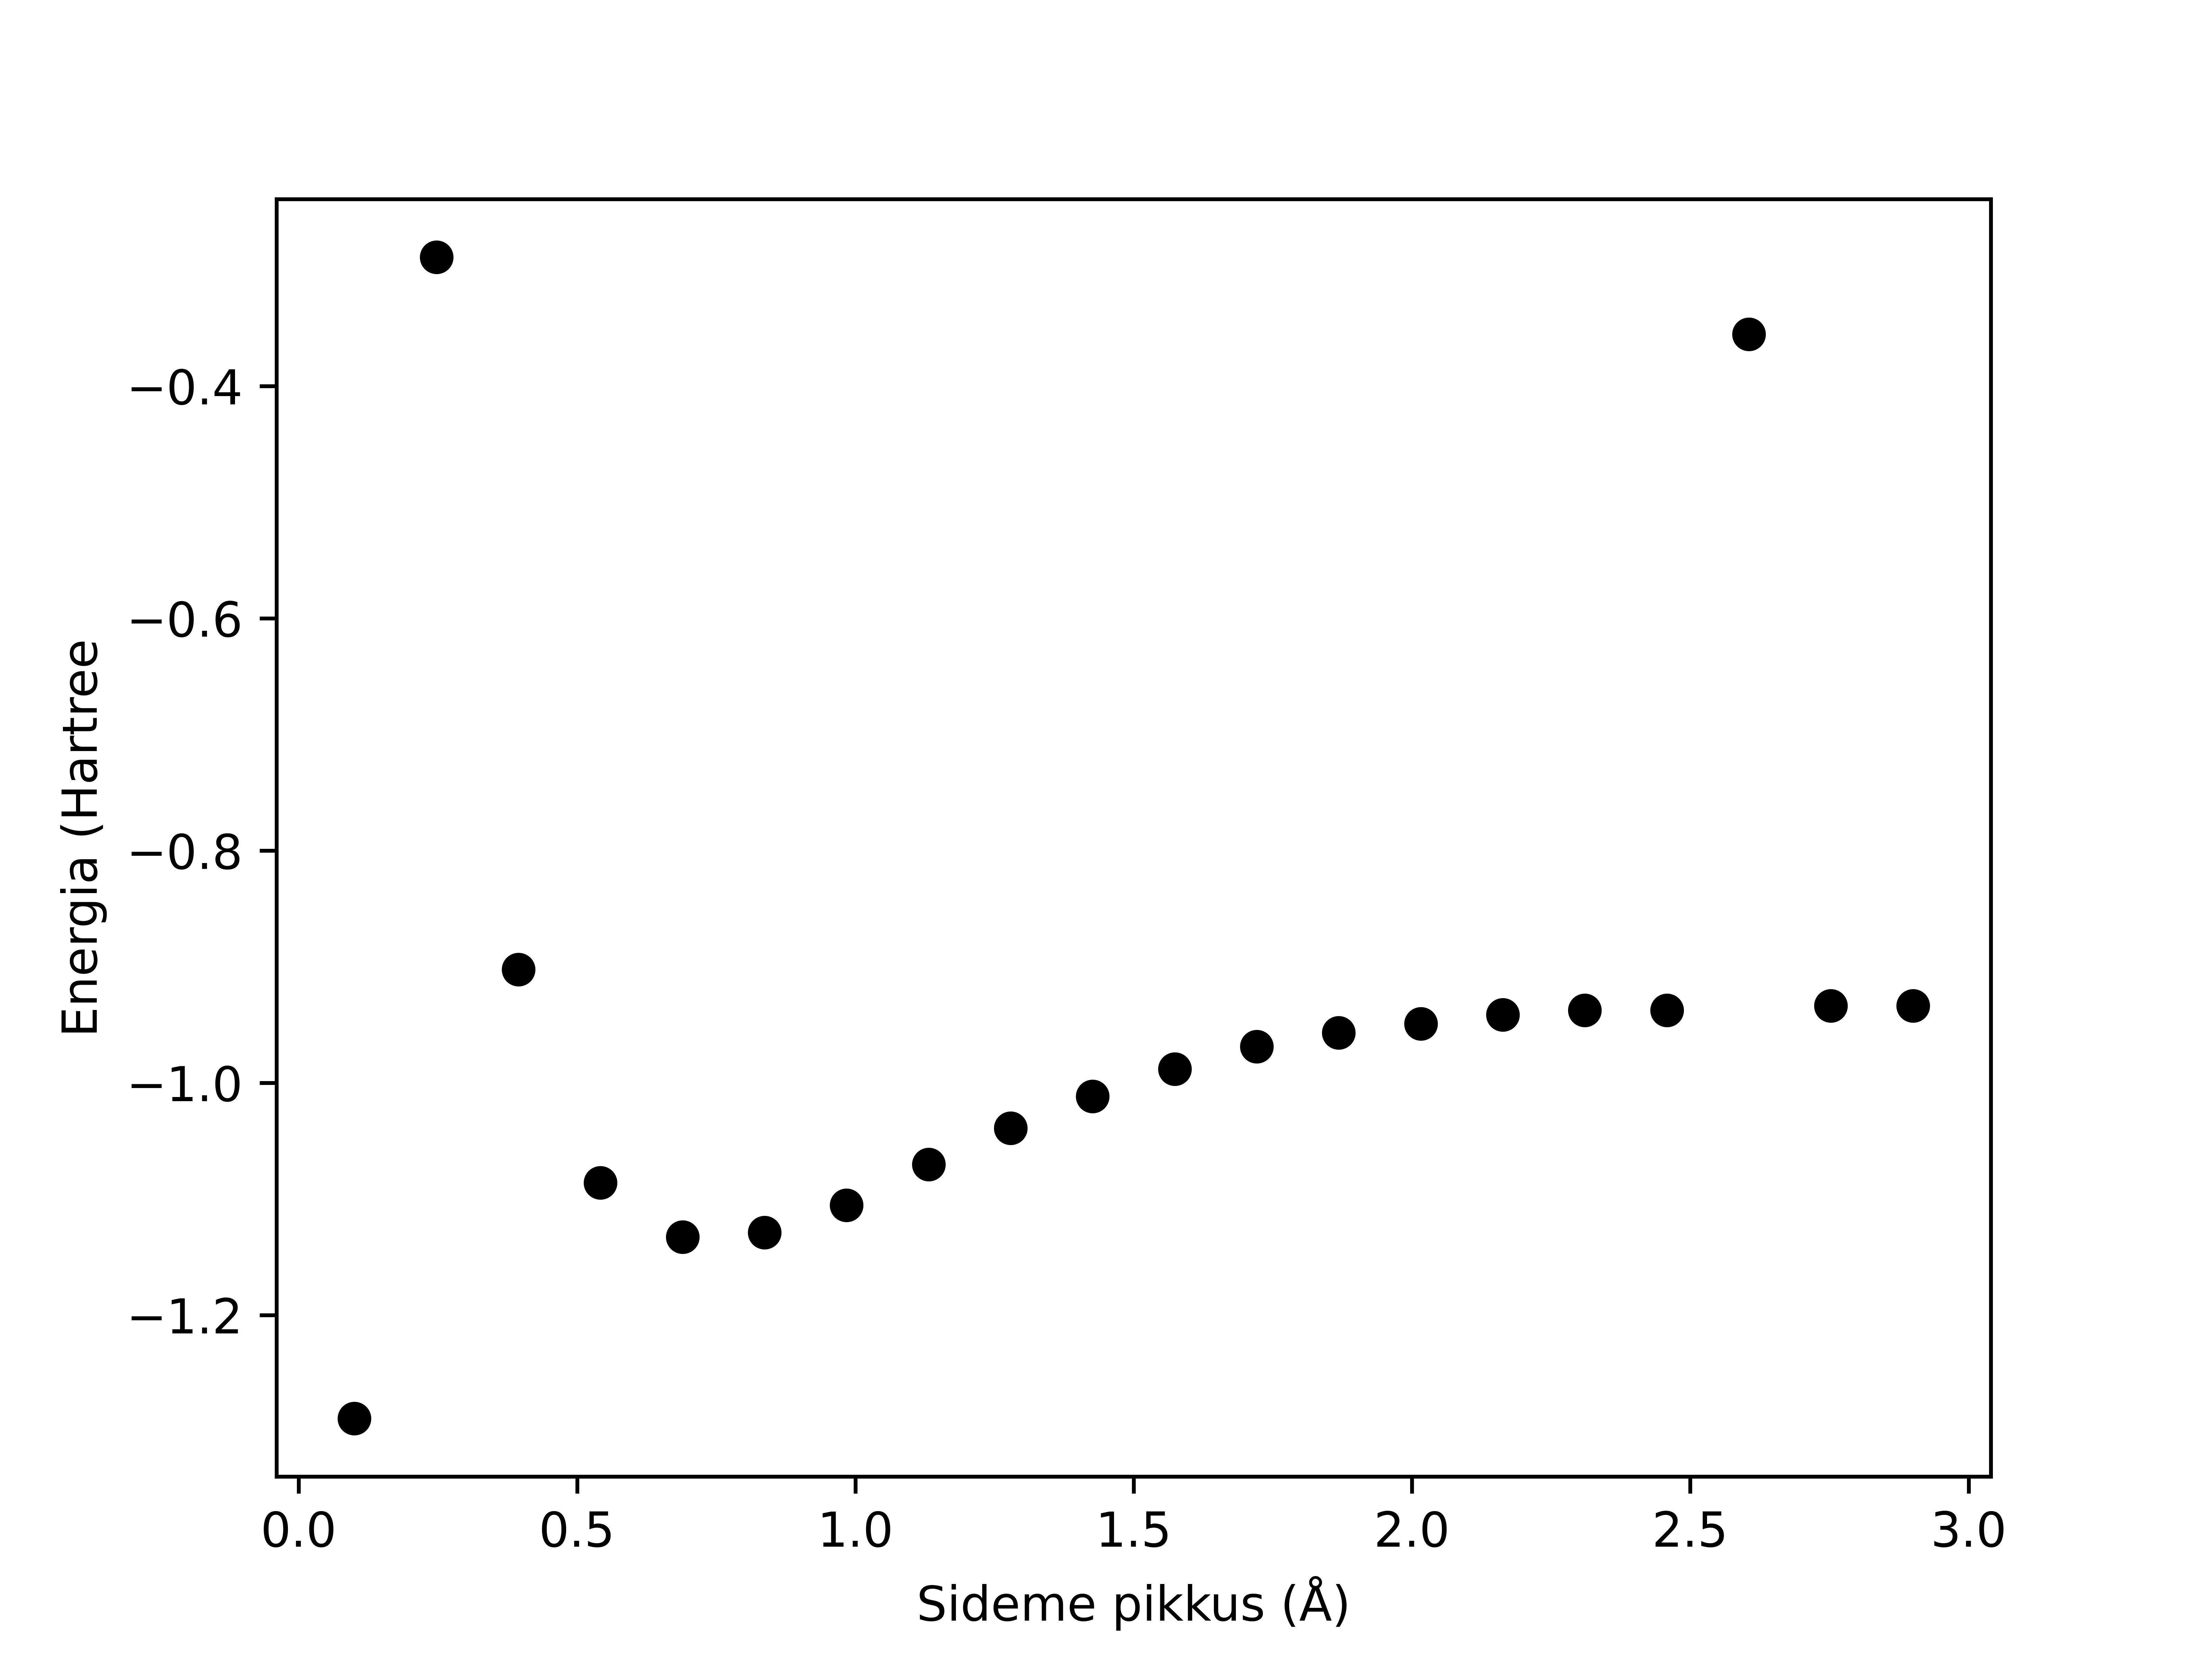
\includegraphics{scan.jpg}
    \caption{Vesiniku elektronkatte energia sõltuvus sideme pikkusest}
    \label{fig:scan}
    \TODO{Joonisel on kaks anomaaliat. Ma ei tea, millest need tulenevad.}
\end{figure}

Joonisel~\ref{fig:scan} on faasi hindamise algoritmi abil saadud energia hinnangu sõltuvus sideme pikkusest.
Iga sideme pikkuse jaoks on vaja koostada eraldi kvantahel ja seda käitada, sest sidemipikkus on hamiltoniaani parameetriks.

Joonise~\ref{fig:scan} jaos leitud energiad on arvutatud 10-kvantbitise täpsusega, 3 trotterisammuga.
Energia ülemiseks piiriks on võetud \(2\,\mathrm{Hartree'd}\).
Nende parameetrite valikut põhjendavad järgnevad jaotised.

\subsection{Trotterisammude arv ja kvantbittide arv}

Sobivate parameetrite leidmist on mõistlik alustada trotterisammude arvu määramisest.

Antud töös proovisime järjest suuremat trotterisammude arvu, kuni sammude arvu suurendamine hinnangut enam ei mõjutanud ja saavatatud oli keemiline täpsus.
Kvantbittide arvu piiras kvantahela käitamise aeg.

\begin{figure}[h]
    \centering
    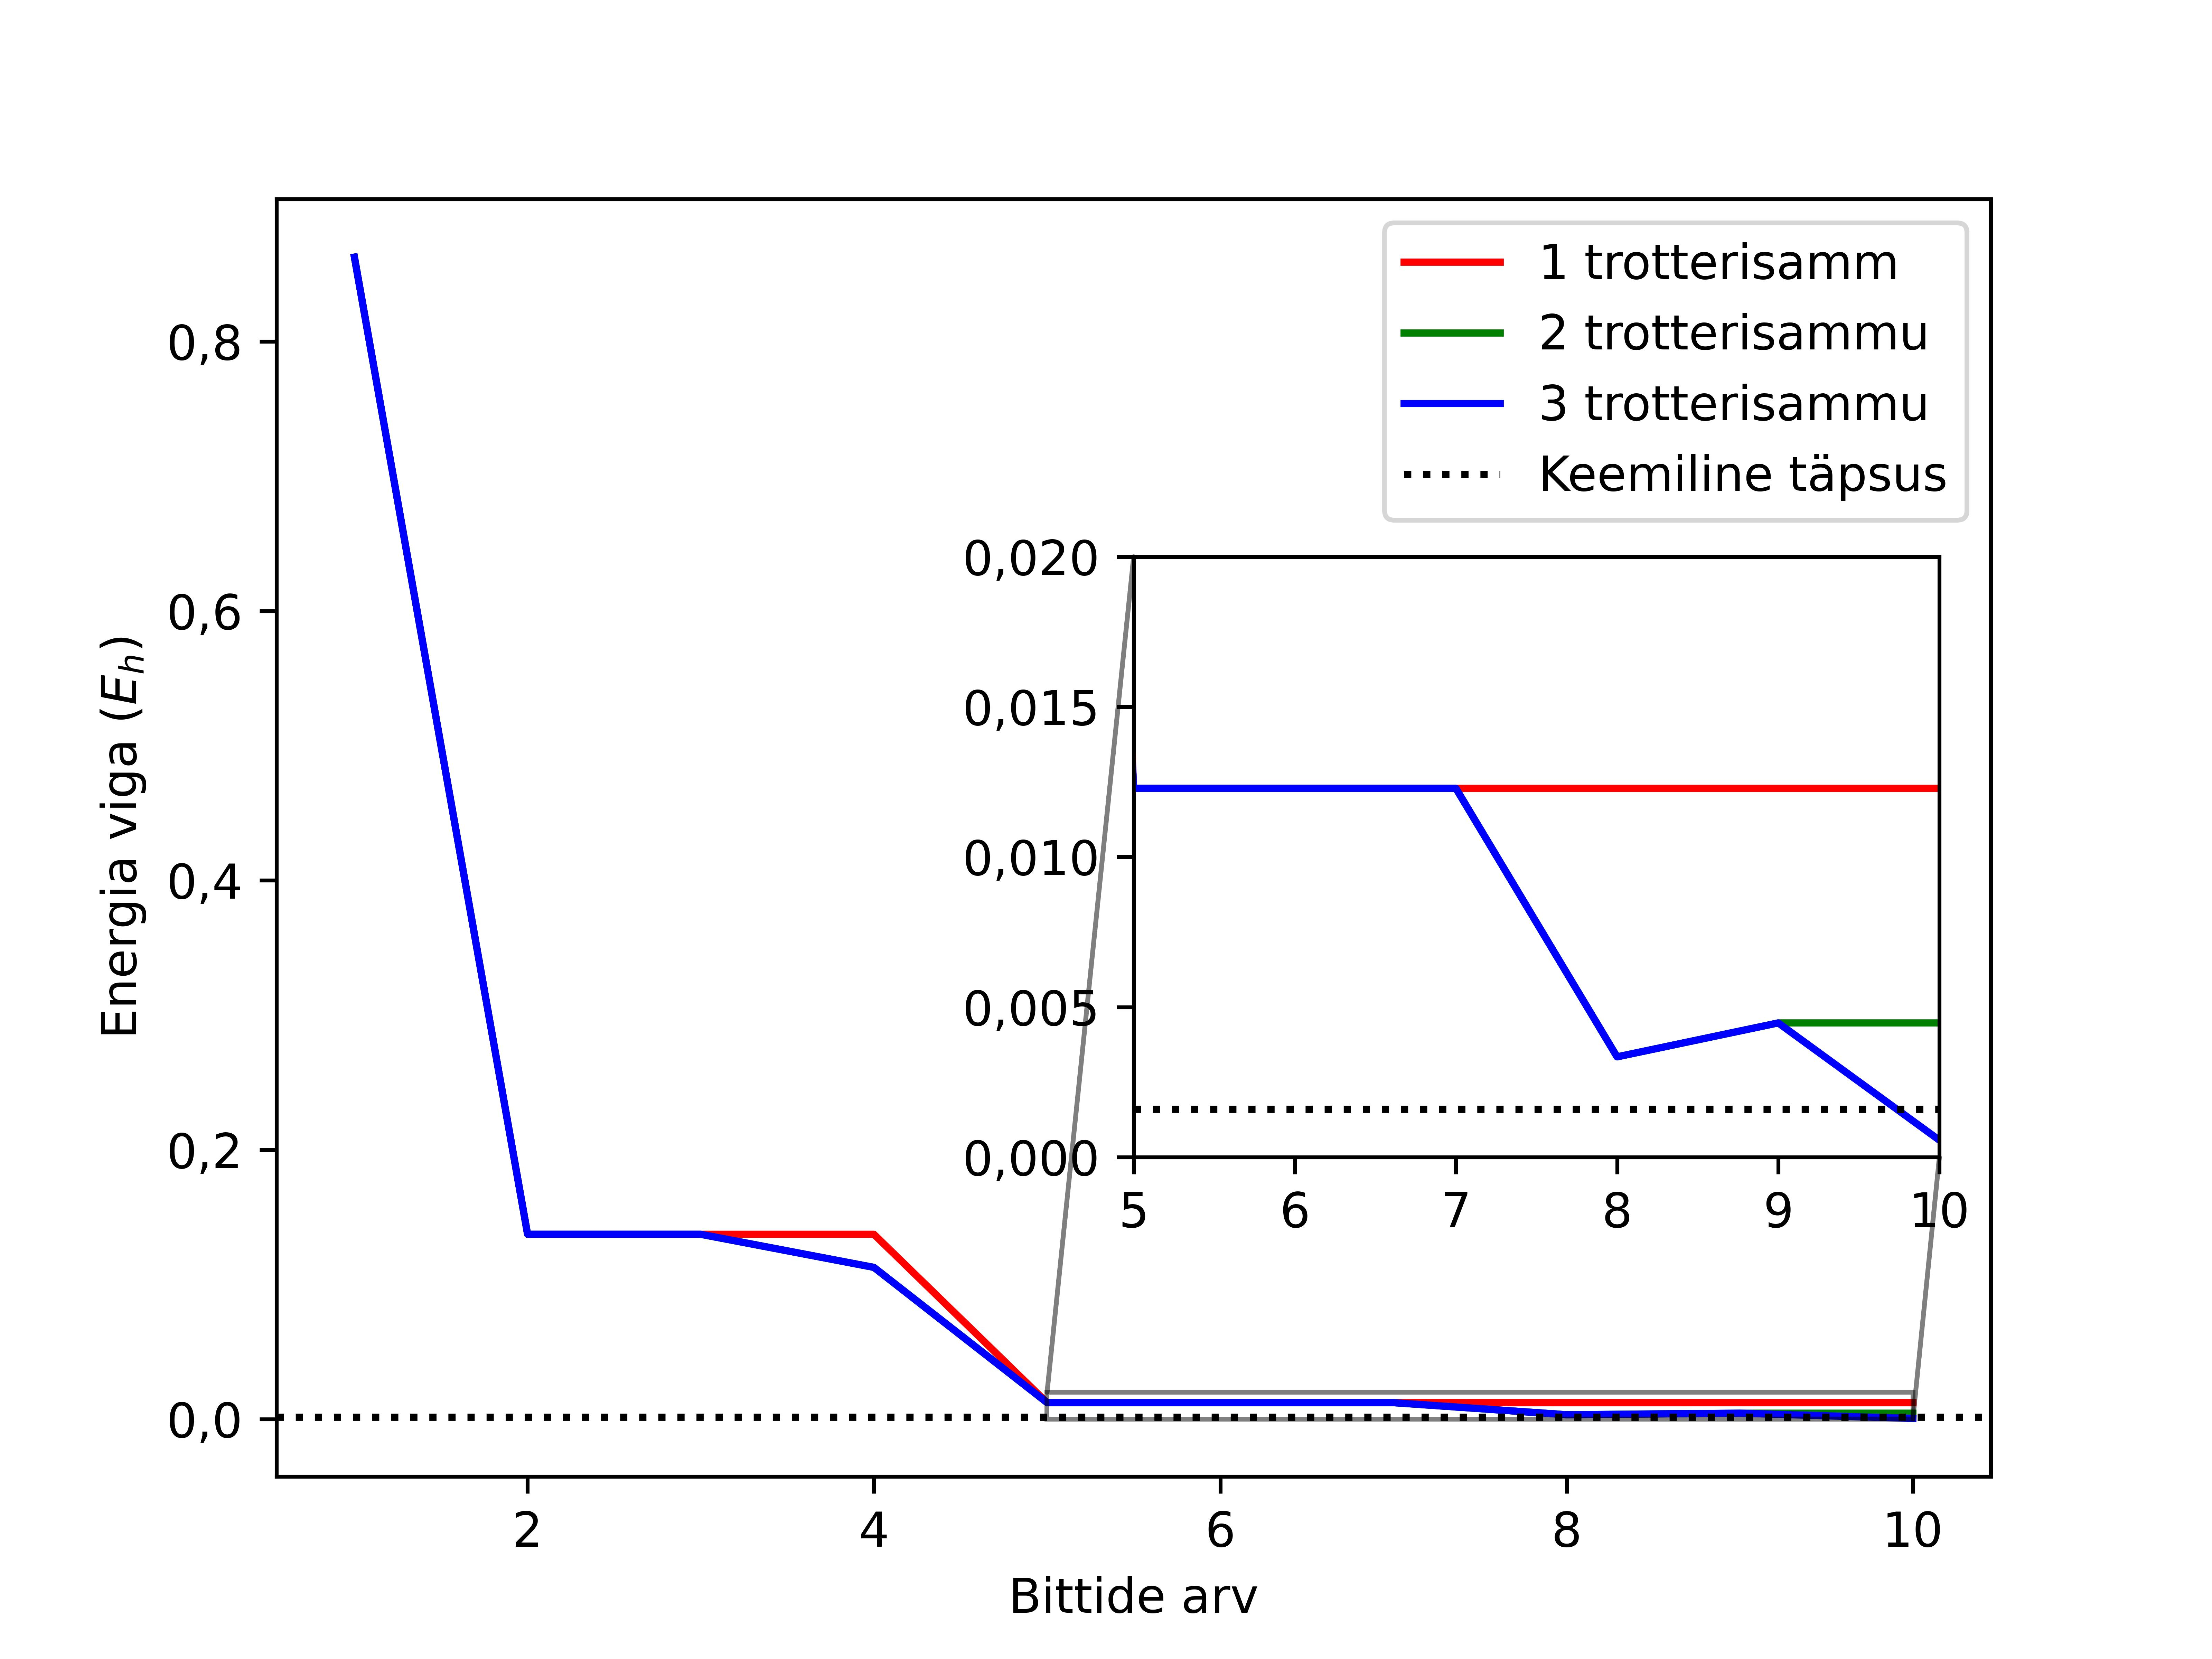
\includegraphics{trotsteps.jpg}
    \caption{Energia hinnangu sõltuvus bittide arvust. Pandagu tähele, et roheline joon on peaaegu täielilt sinese joone taga varjatud}
    \label{fig:trotsteps}
\end{figure}

Nagu näha jooniselt~\ref{fig:trotsteps} langevad ühe-, kahe- ja kolme-trotterisammused energia hinnangud hästi kokku juhul, kui energiat hinnata kahekse- või vähemakvantbitise täpsuega.
Erinevused ilmnevad alles kahekasst kvantbitist suurema täpsuse juures.
Keemiline täpsuse saavutasime kolme trotterisammu ja kümne kvantbitiga.

Parimal juhul on võimalik saavutada vaid nii suur täpsus, kui keemilise baasi valik lubab.

Trotterisammude arvu suurendamisel kasvab ahela pikkus ja seega ka kätamisaeg eksonentsiaalselt.

Kvantbittide arvust sõltub käitamisaeg kahte moodi.
Esiteks, rohkem kvantbitte tähendab pikemat käitamisaega.
Teiseks, kui faasi hindamiseks kasutada rohkem kvantbitte, siis kasvab eksponentsiaalselt ka ahela pikkus.

\begin{figure}[h]
    \centering
    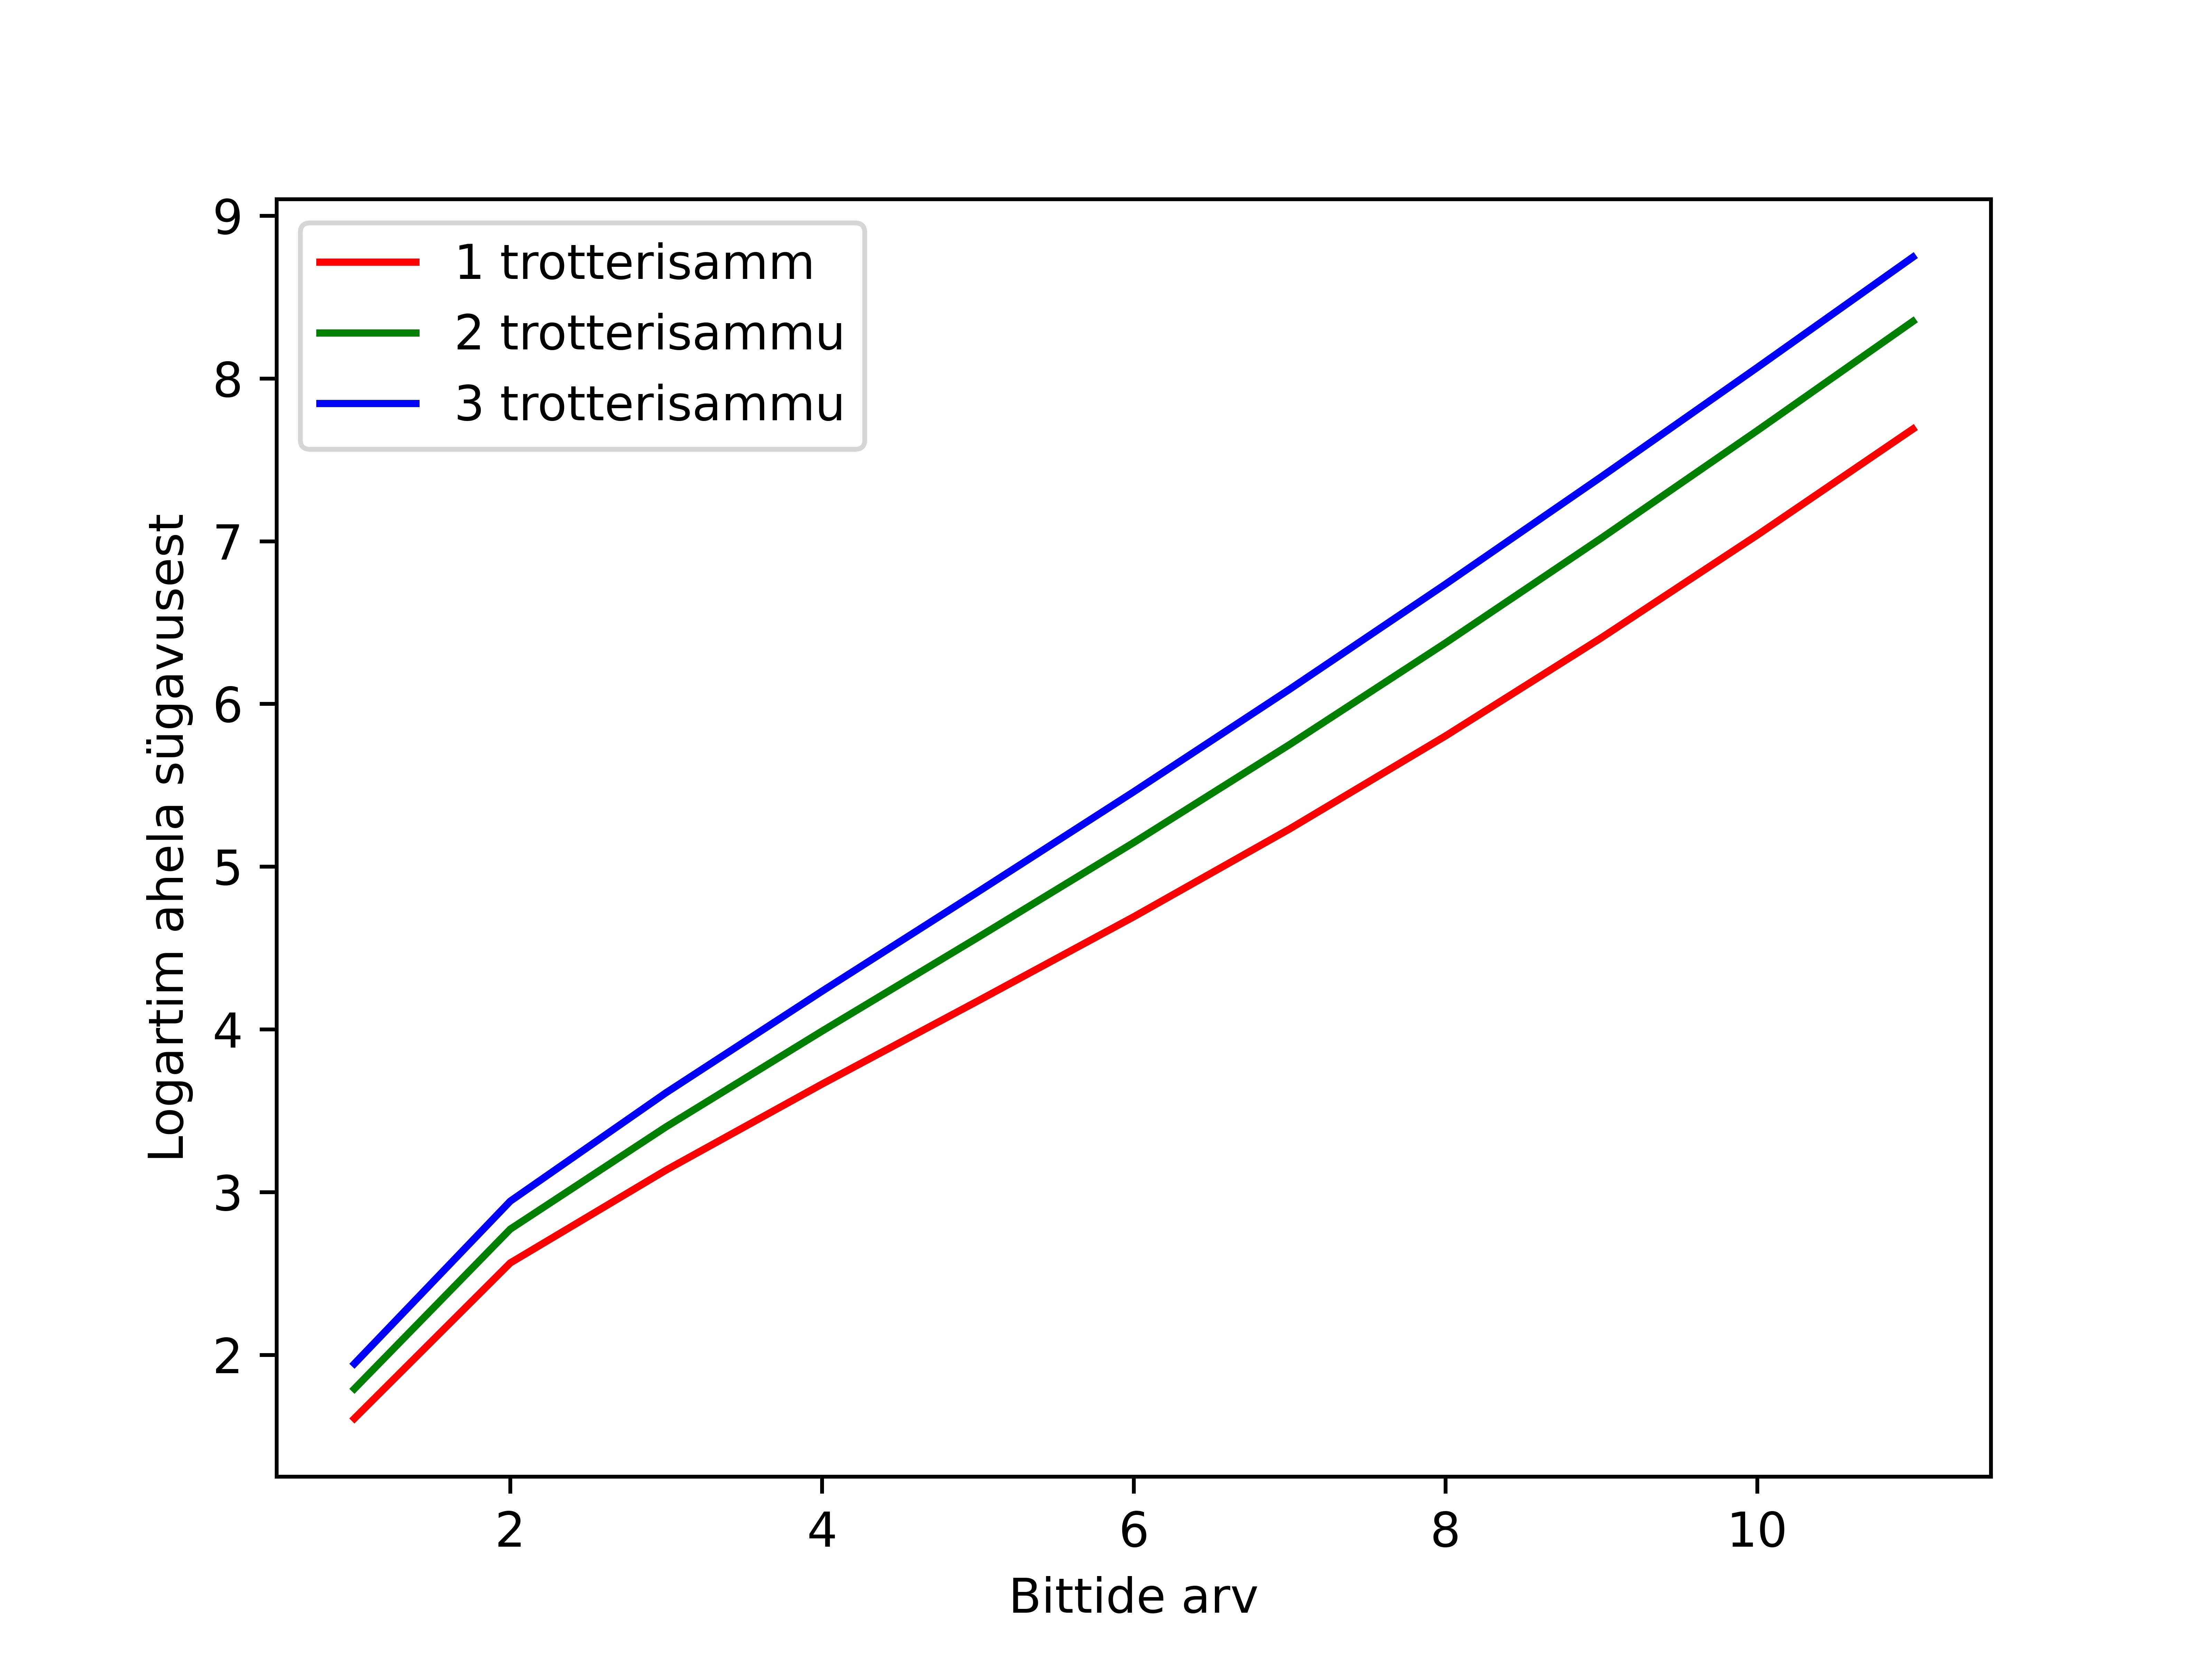
\includegraphics{depths.jpg}
    \caption{Ahela sügavuse sõltuvs bittide arvust}
    \label{fig:depths}
\end{figure}

Joonisel~\ref{fig:depths} on näidatud ahela sügavuse, st ahelas olevat kvantväravate arvu, sõltuvus kvantbittide arvust erinevat trotteri sammude arvu jaoks.
Praktiliselt on teostatav kümne kvantbiti kasutamine.

\subsection{Eneriga piirväärtus}

Samuti sõltub energia hinnangu täpsus energia piirväärtuse valikust, mida kujutab joonis~\ref{fig:bounds}.

\begin{figure}[h]
    \centering
    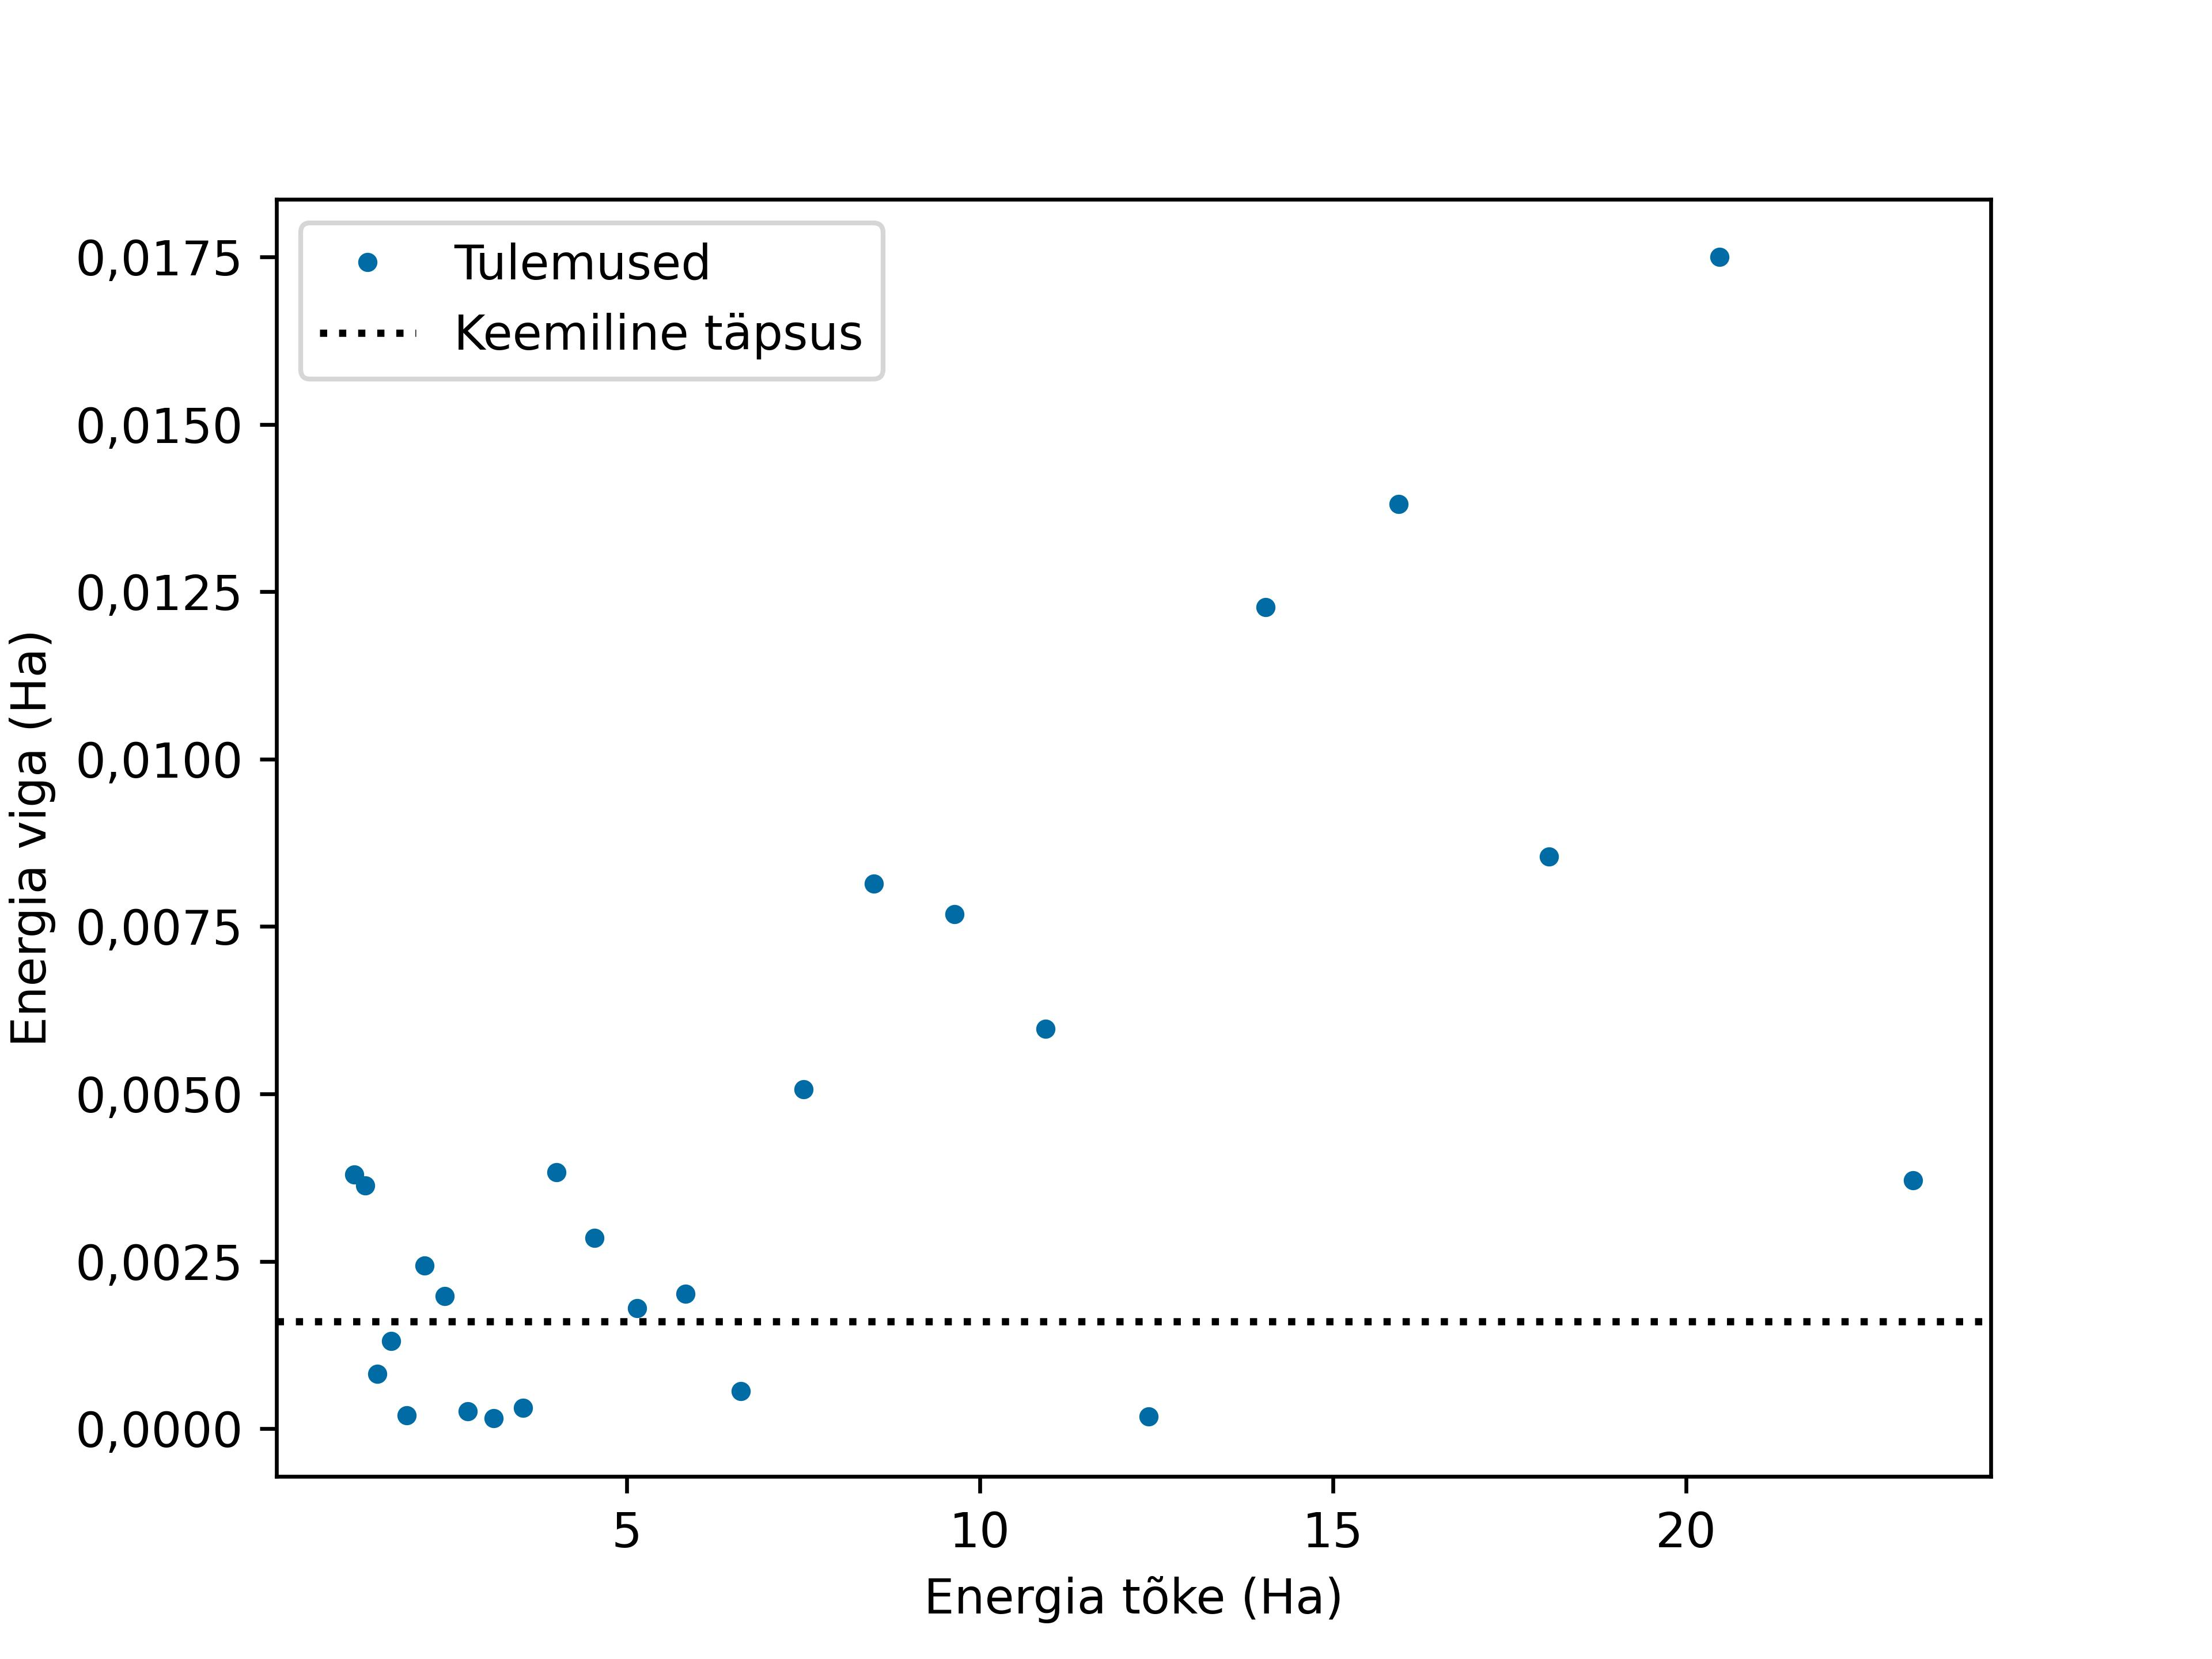
\includegraphics{bounds.jpg}
    \caption{Energia hinnagu sõltuvus energia piirväärtuse valikust}
    \label{fig:bounds}
\end{figure}

Nagu näha, sõltub energia hinnagu täpsus piirvääruse valikust kaootiliselt.
Siiski energiast oluliselt suuremate piirväärtuste puhul (mida joonisel~\ref{fig:bounds} pole kujutatud), täpsus reeglina väheneb.
Nimelt on sellisel juhul \(\phi \ll 1\) ja seega ei panusta esimesed kvantbitid tulemuse täpsusesse.

\subsection{Edasiarendusi}

Faasi hindamise algoritmi peamine edasiarendus on iteratiivne faasi hindamise algoritm~\cite{mcardle+etal, omalley+etal}.

Tegemist on hübriidalgoritmiga, mis kasutab klassikalist ja kvantarvutit vaheldumisi.
Kvantarvutuslikult loetakse välja üks bitt korraga, mille põhjal koostatakse klassikaliselt uus ahel järgmise biti välja lugemiseks.

Sellise algoritmi eeliseks on, et faasi hindamise registrisse on vaja vaid ühte kvantbitti.
Samuti on ahelad lühemad.

Puuduseks on keerulisus ja asjaolu, et võimalik viga mõne biti välja lugemisel võib kumuleeruda.

\TODO{Mida siin veel öelda?}

\nonumsection{Kokkuvõte}

\clearpage\newpage\addcontentsline{toc}{section}{Kirjandus}\printbibliography[title=Kirjandus]

\end{document}
